\documentclass[border=6pt]{standalone}
\usepackage{tikz}
\usetikzlibrary{arrows.meta, positioning}

\definecolor{gene}{HTML}{0072B2}
\definecolor{eff}{HTML}{009E73}

\begin{document}
\pagecolor{white}
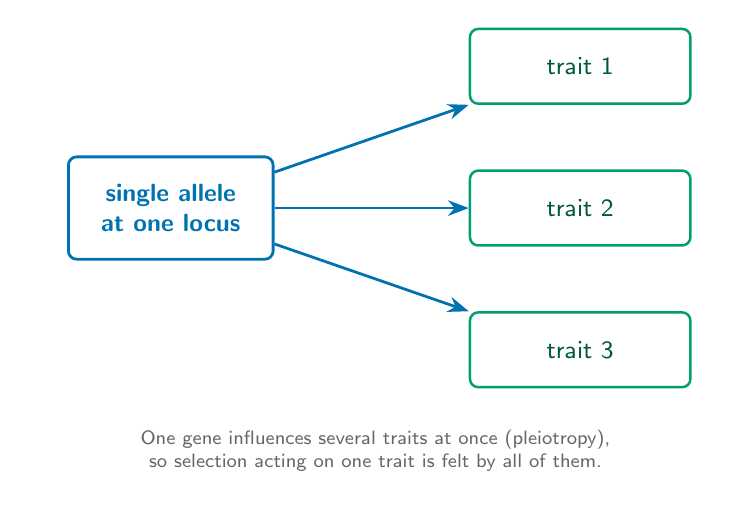
\begin{tikzpicture}[
    >=Stealth, font=\sffamily,
    lab/.style={font=\sffamily\scriptsize, text=black!60, align=center},
    gnode/.style={draw=gene, text=gene, rounded corners=3pt, line width=1.0pt,
                  align=center, minimum width=2.6cm, minimum height=1.3cm,
                  font=\sffamily\small\bfseries},
    enode/.style={draw=eff, text=eff!55!black, rounded corners=3pt, line width=0.9pt,
                  align=center, minimum width=2.8cm, minimum height=0.95cm,
                  font=\sffamily\small},
]
\node[gnode] (g) at (0,0) {single allele\\ at one locus};

\node[enode] (e1) at (5.2, 1.8)  {trait 1};
\node[enode] (e2) at (5.2, 0)    {trait 2};
\node[enode] (e3) at (5.2, -1.8) {trait 3};

\draw[->, line width=1.0pt, gene] (g) -- (e1);
\draw[->, line width=1.0pt, gene] (g) -- (e2);
\draw[->, line width=1.0pt, gene] (g) -- (e3);

\node[lab, anchor=north, text width=8.6cm] at (2.6,-2.7)
   {One gene influences several traits at once (pleiotropy),\\
    so selection acting on one trait is felt by all of them.};

\end{tikzpicture}
\end{document}
